% Chapter 1

\chapter{Building Datasets} % Main chapter title

\label{Chapter2} % For referencing the chapter elsewhere, use \ref{Chapter1} 

%----------------------------------------------------------------------------------------

% Define some commands to keep the formatting separated from the content 
\newcommand{\keyword}[1]{\textbf{#1}}
\newcommand{\tabhead}[1]{\textbf{#1}}
\newcommand{\code}[1]{\texttt{#1}}
\newcommand{\file}[1]{\texttt{\bfseries#1}}
\newcommand{\option}[1]{\texttt{\itshape#1}}

In this chapter, we will give an overview of existing (labelled) aerial imagery datasets and outline the reasons why none of them is suitable for our investigation. Following this discussion, we will describe two approaches for obtaining our own labelled dataset.

\section{Requirements and Considerations}

Before we go into the presentation of already existing labelled datasets we discuss the requirements that the dataset needs to fulfill in order to serve for the investigation in this thesis project. As a refresher, we want to detect human impact on aerial images and determine the dependency of a chosen evaluation metric on resolution per pixel. Ideally, the range for the resolutions should scale from a few tens of centimeters to a few tens of meters, whereas the images with low resolution can be generated from the high resolution images by downsampling. \textcolor{red}{TODO: Explain degradation process.} Having in mind previous arguments, we mainly need to consider three aspects. 

First, we need to have imagery data with labels that can be used to clearly distinguish between existing and non-existing human impact on the images, respectively. This impact might be classified pixel wise, or as binary classification for the entire image, or as multi-class classification that can be translated into binary labelling. Second, 
we need a balanced dataset of approximately the same number of images for both labels, and a as large as possible variation of the images with respect to different terrains. Third, the images need to have a resolution per pixel which is equal or better than 1m. Also, the height and width of the images should measure at least $500\times500$ pixels, so that one has enough room for degradation. 

\section{Existing Datasets}

In literature, there can be found several remote sensing datasets with ground truth labels. We have listed the most relevant ones in table \ref{table:datasets}. The table first lists the name of the dataset together with the bibliogrpahic reference. It also details the data source for the images. Further it contains the number of images, the resolution of the images, the size (in pixel) of the images where images are squared, and the number of categories.

The datasets were collected using different publicly available data sources. These range from pure low resolution satellite imagery (Sentinel-2) to high-resolution images taken with an aircraft (USGS) to a mix of different image sources (Google Earth). 

\begin{table}[h!]
	\begin{tabular}{l | l | l | l | l | l }
	name & source & images & resolution (m) & size (pixel) & categories \\
	\hline
	BigEarthNet \parencite{sumbul2019} & Sentinel-2 & 590,326 & 10, 20, 60 & 120, 60, 20 & $\sim$ 50 \\
	EuroSAT \parencite{helber2017}	& Sentinel-2 & 27,000  & 10 & 64  & 10 \\
	UCMerced \parencite{yang2010} & USGS & 2100 & 0.3 & 256 & 21 \\
	DeepSat \parencite{basu2015}  & USGS  & 405,000 & 1 & 28 & 6  \\
	AID \parencite{xia2016} & Google Earth & 10,000  & 0.5 - 8  & 600 & 30 \\
	PatternNet \parencite{zhou2017} & Google Earth & 30,400 & 0.06 - 4.69 & 256 & 38 \\
	\end{tabular}
	\caption{Publicly available remote sensing datasets with labels.}
	\label{table:datasets}	
\end{table}

The satellite images have a resolution of equal or larger than 10~m and they are collected with the Sentinel-2 satellites of the European Earth observation program Copernicus. Although the datasets from this source (BigEarthNet and EuroSat) are comparatively large, they do not suffice for our purpose, because the resolution is not good enough and the images are too small.

The USGS National Map Urban Area Imagery collection \href{https://earthexplorer.usgs.gov/}{(\textit{see link})} was utilized to collect a remote sensing dataset by the two works UCMerced and DeepSat, where the former is the dataset that comes closest to our requirements. It has 21 categories of which only 2 belong to images without human impact, while the other 19 show human impact. The DeepSat dataset unfortunately consists of image patches which are only $28 \times 28$ large, so that we aren't able to study these images as a function of resolution.

The datasets using Google Earth as data source are collected using either the Google Earth or the Google Maps API. These images vary in resolution as well as in their original data provider since Google accesses several data sources. 
Both datasets, the AID and the PatternNet dataset, have about 30 categories with several images in each category. Here, different categories have different resolutions per pixel, and again most of the categories relate to urban areas so that we do not have sufficient images without human impact. Even the categories that in principle should not show human influence contain images that break this rule.

Overall, the main issue with these datasets stems from the fact that non of them was collected with the purpose to analyze human impact and therefore they are very unbalanced, and do not contain sufficient variety of images for the  label no-human impact. Therefore, we decided to collect and label images by ourselfes. In our first approach we used the Google Maps API.

\section{Google Maps}

...

\section{USGS, Land Cover}

\subsection{Getting the Data}
To be able to construct a balanced and representative dataset we first decided to focus on images of the United States, which allows for a large variety of different terrains. We then used as data source the Aerial Imagery datasets from USGS Earthexplorer \href{https://earthexplorer.usgs.gov/}{(\textit{see link})} which we combined with information about Land Cover and Land Use available from the USGS Land Cover Viewer \href{https://gis1.usgs.gov/csas/gap/viewer/land_cover/Map.aspx}{(\textit{see link})}.

When looking for images we excluded cities and highly developed urban areas, and instead focussed on unpopulated areas. Specifically, we limited our image search to the four Land Use categories
\begin{itemize}
	\item Agriculture
	\item Shrubland-Grassland
	\item Semi-Desert
	\item Forest-Woodland
\end{itemize}
that can be found in the USGS Land Cover Viewer. Note that these categories served as a rough geographic reference to pin down geolocations of interest, in order to guarantee a dataset with a good variety of different terrains. We also found that it is harder to find images without human, which is why we selected many images from national parks. However, within a given area/terrain we always tried to have images with and without impact.

Once an area was pointed out as a region of interest, we located it on USGS Earthexplorer and downloaded images from that area. In particular, we constructed two datasets with $0.3m$ and $1m$ resolution, respectively. The former was taken from the category High Resolution Orthoimagery and the latter from the category National Agriculture Imagery Program (NAIP). Note that the images in these categories usually have a height and a width of several thousand pixels, and hence oocupy a few hundreds of Megabytes of disk space. We cropped smaller images out of the raw images, which will be discussed in more detail in the following section. Overall, we downloaded about 100 images for each dataset.


\subsection{Data Processing and Labeling}
Our data processing pipeline consists of the following steps:
\begin{itemize}
	\item Download large raw images
	\item Crop images of size $512\times512$ pixels
	\item Labelling the images with either 0 (no human impact) or 1 (human impact)
	\item Degrading the images, i.e. reducing the number of pixels
\end{itemize}

\textcolor{red}{TODO: mention all the scripts/notebooks for the respective parts}

Let us discuss each of these steps in more detail. Every raw image was processed, whereas the processed images of size $512\times512$ were saved in a folder named by its category. Note that every raw image resulted in approximately $100 - 150$ processed images, so that we ended up with more than 10,000 images for each dataset.

\begin{figure}%[th]
	\centering
	\captionsetup{width=1\linewidth}
	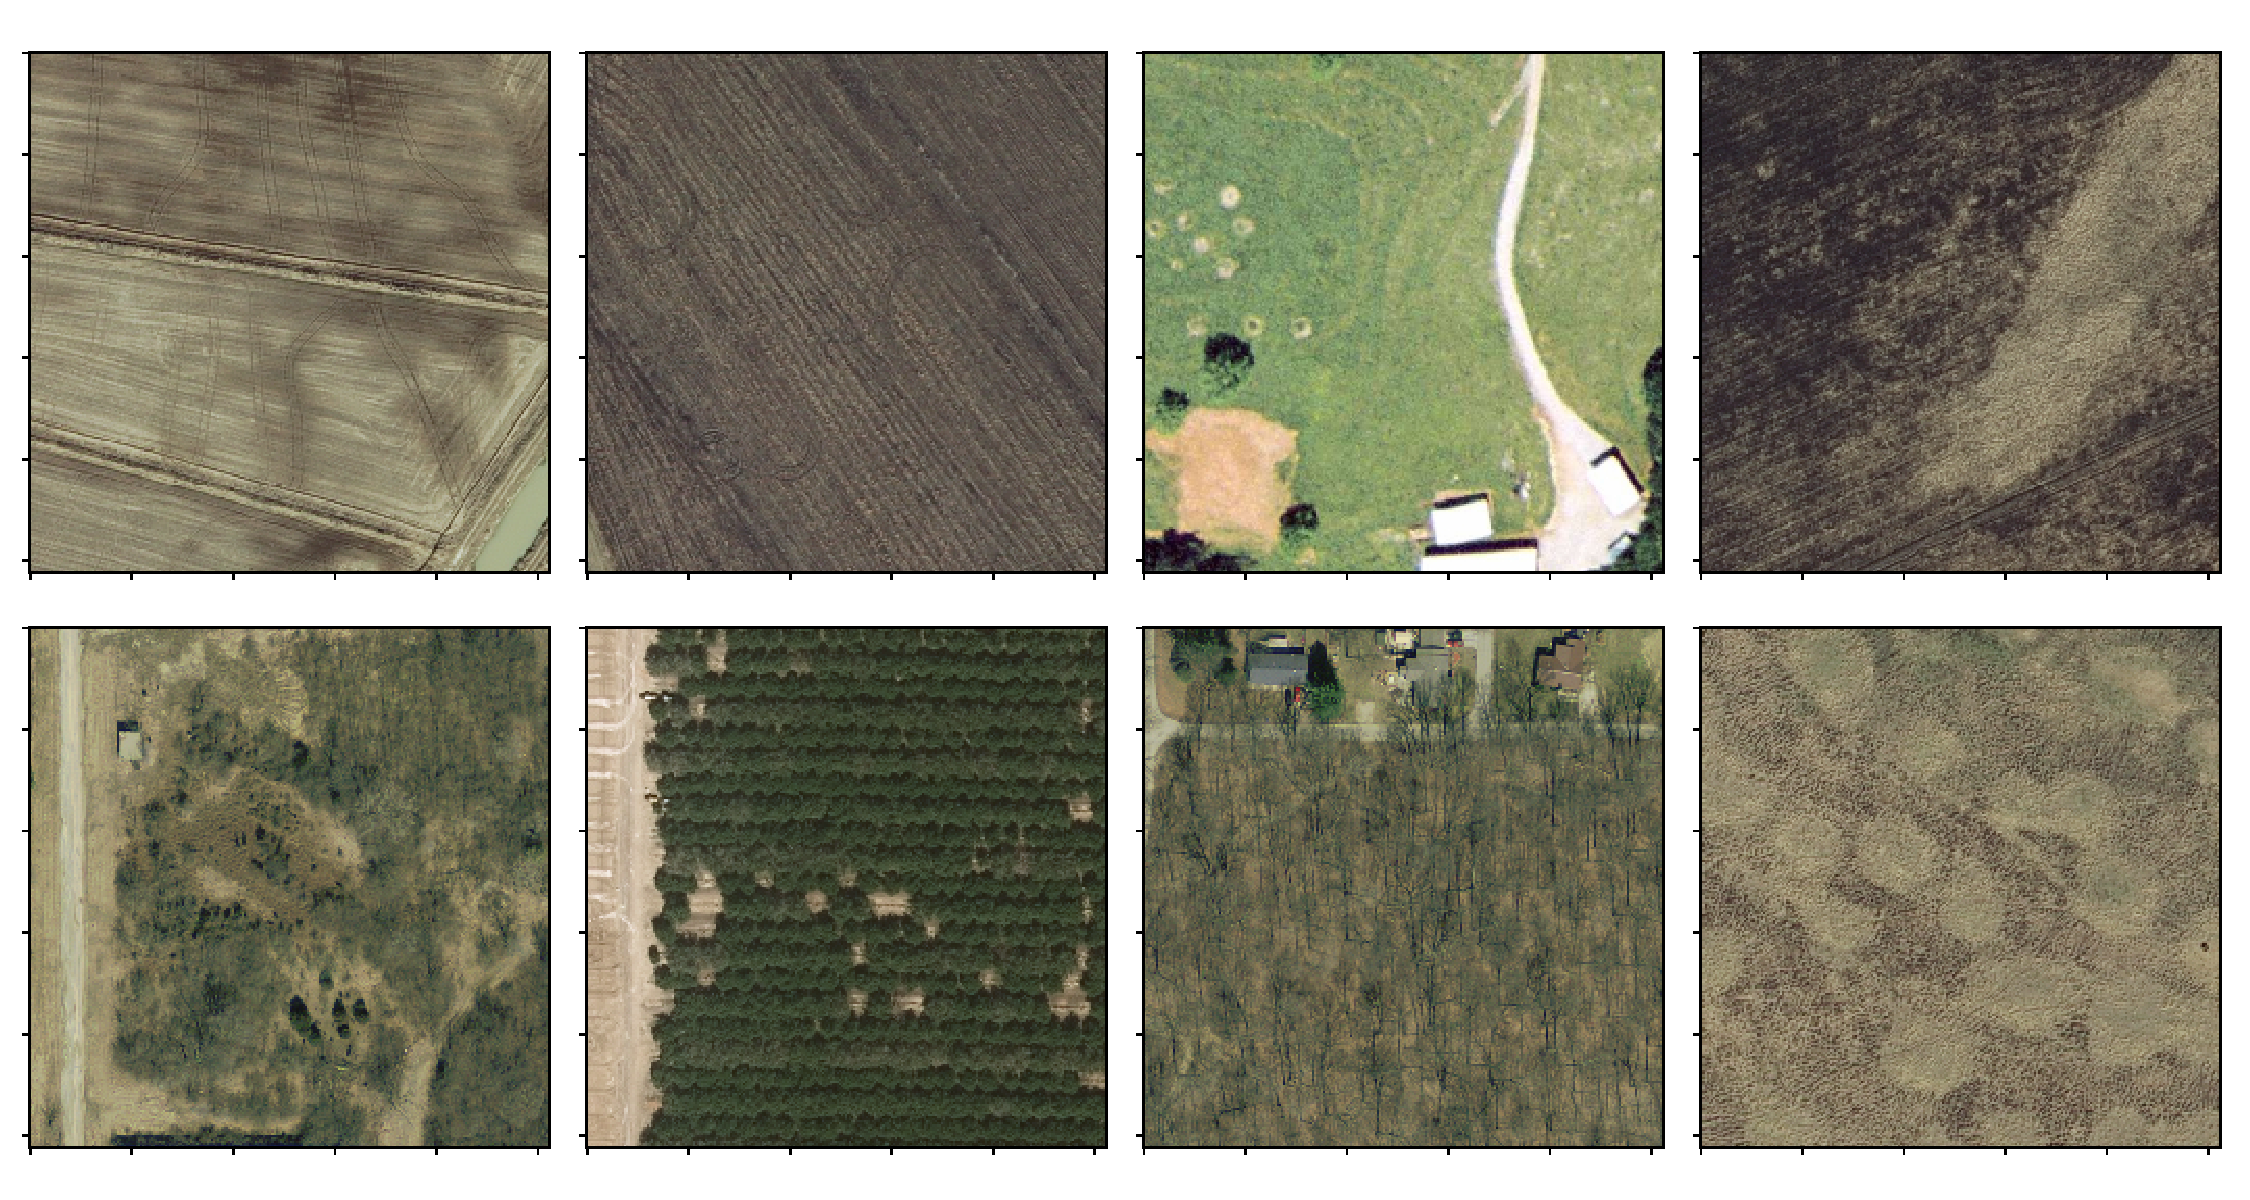
\includegraphics[width=1\textwidth]{Figures/agriculture_sample.pdf}
	\caption{\textbf{Example images of category Agricultue.} All images in this figure show clear signs of human impact. The images in this figure have a size of $512\times512$ pixels and a resolution of $0.3$m per pixel.}
	\label{fig:agriculture_sample}
\end{figure}

\begin{figure}%[th]
	\centering
	\captionsetup{width=1\linewidth}
	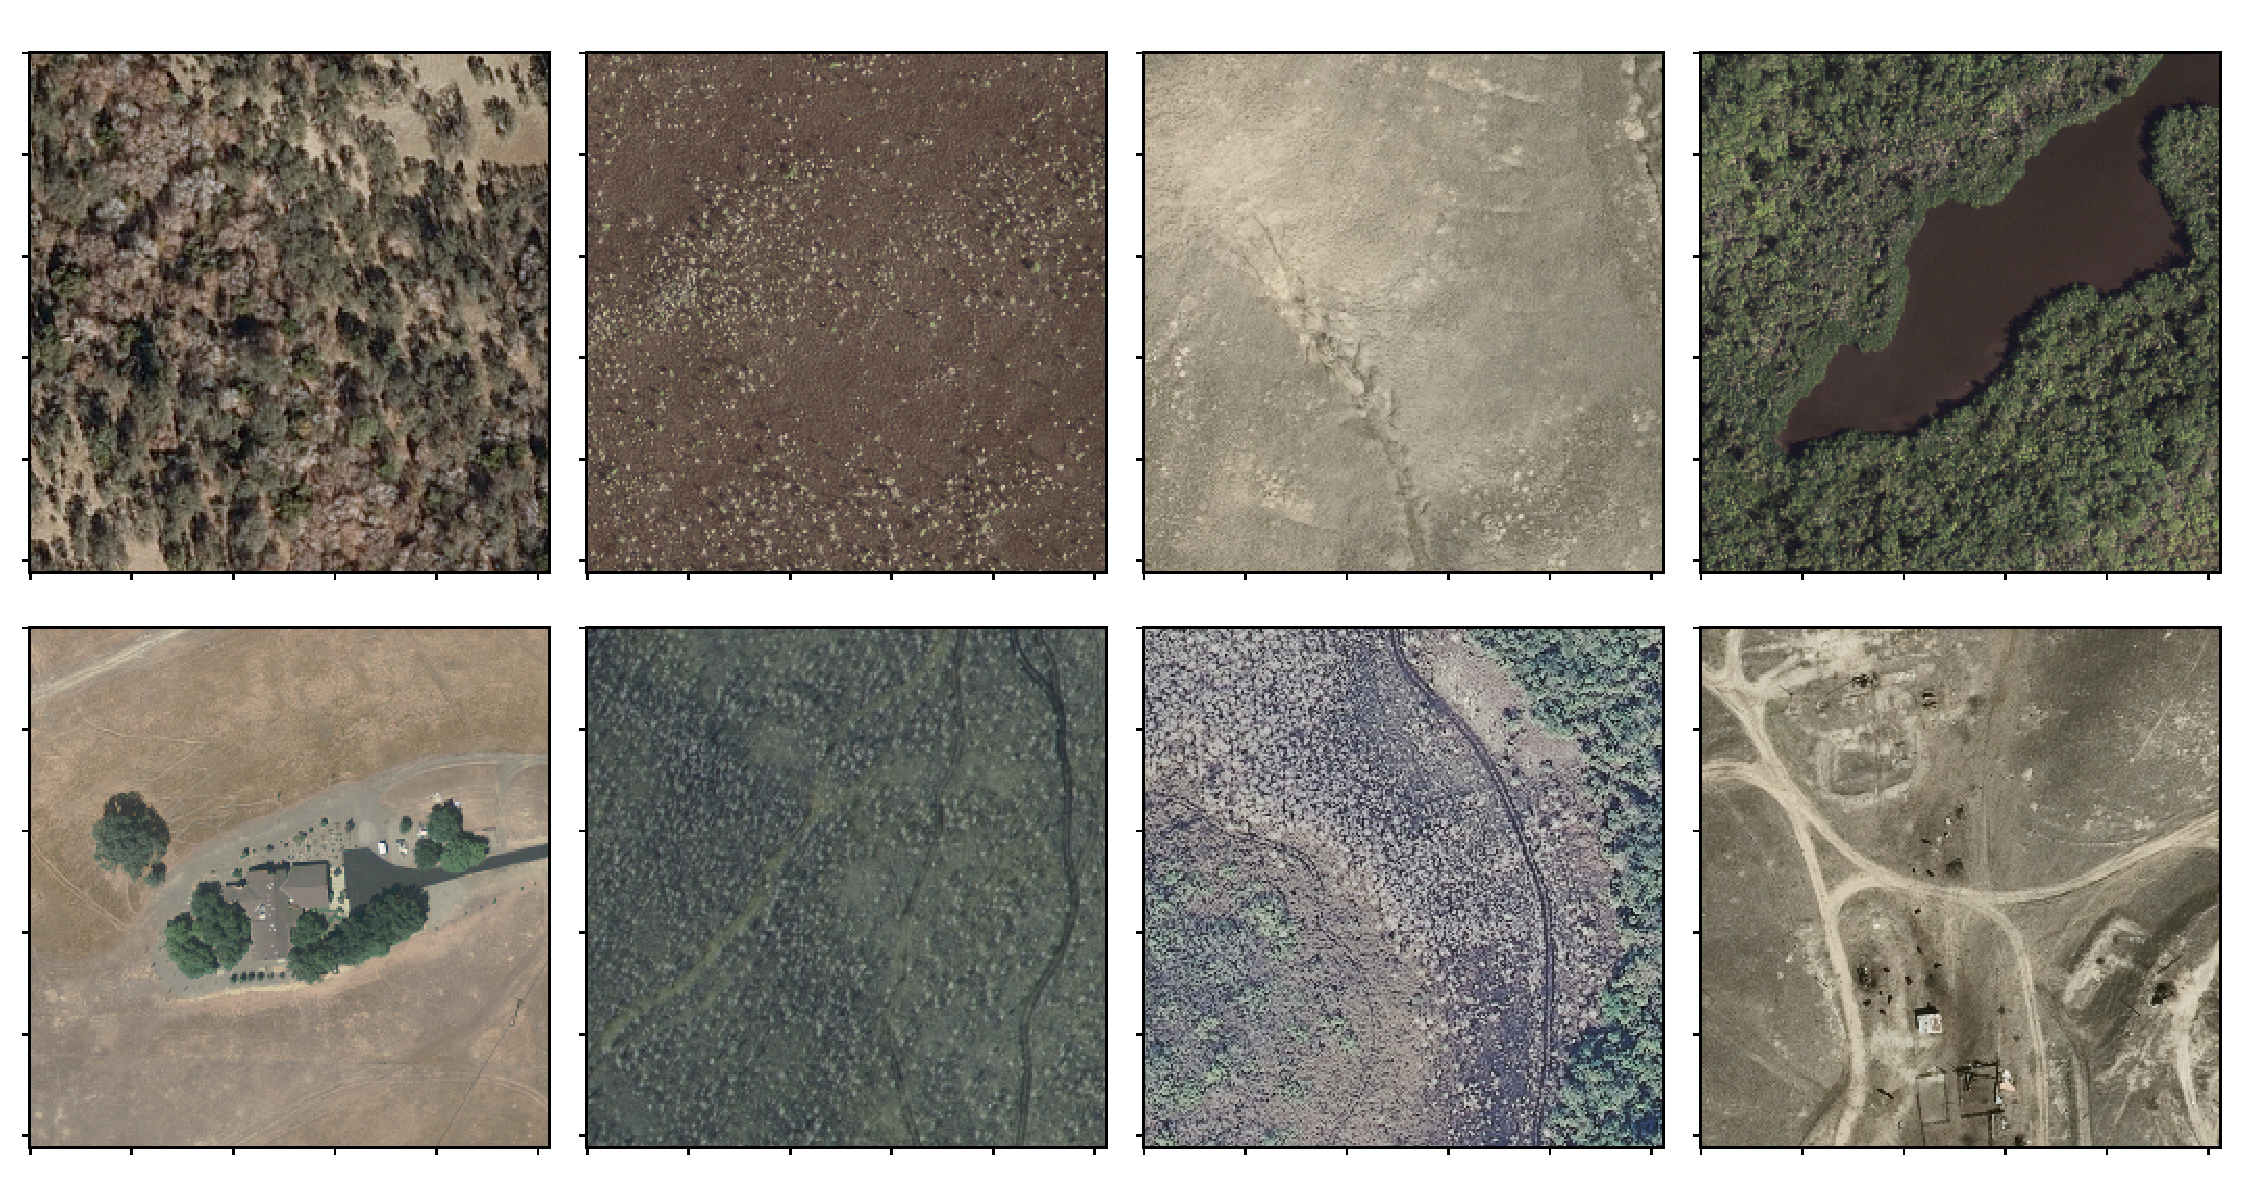
\includegraphics[width=1\textwidth]{Figures/shrubland-grassland_sample.pdf}
	\caption{\textbf{Example images of category Shrubland-grassland.} The images in the first row do not contain any human influence, while the images in the second row show influence by humans. The images in this figure have a size of $512\times512$ pixels and a resolution of $0.3$m per pixel.}
	\label{fig:shrubland-sample}
\end{figure}

\begin{figure}%[th]
	\centering
	\captionsetup{width=1\linewidth}
	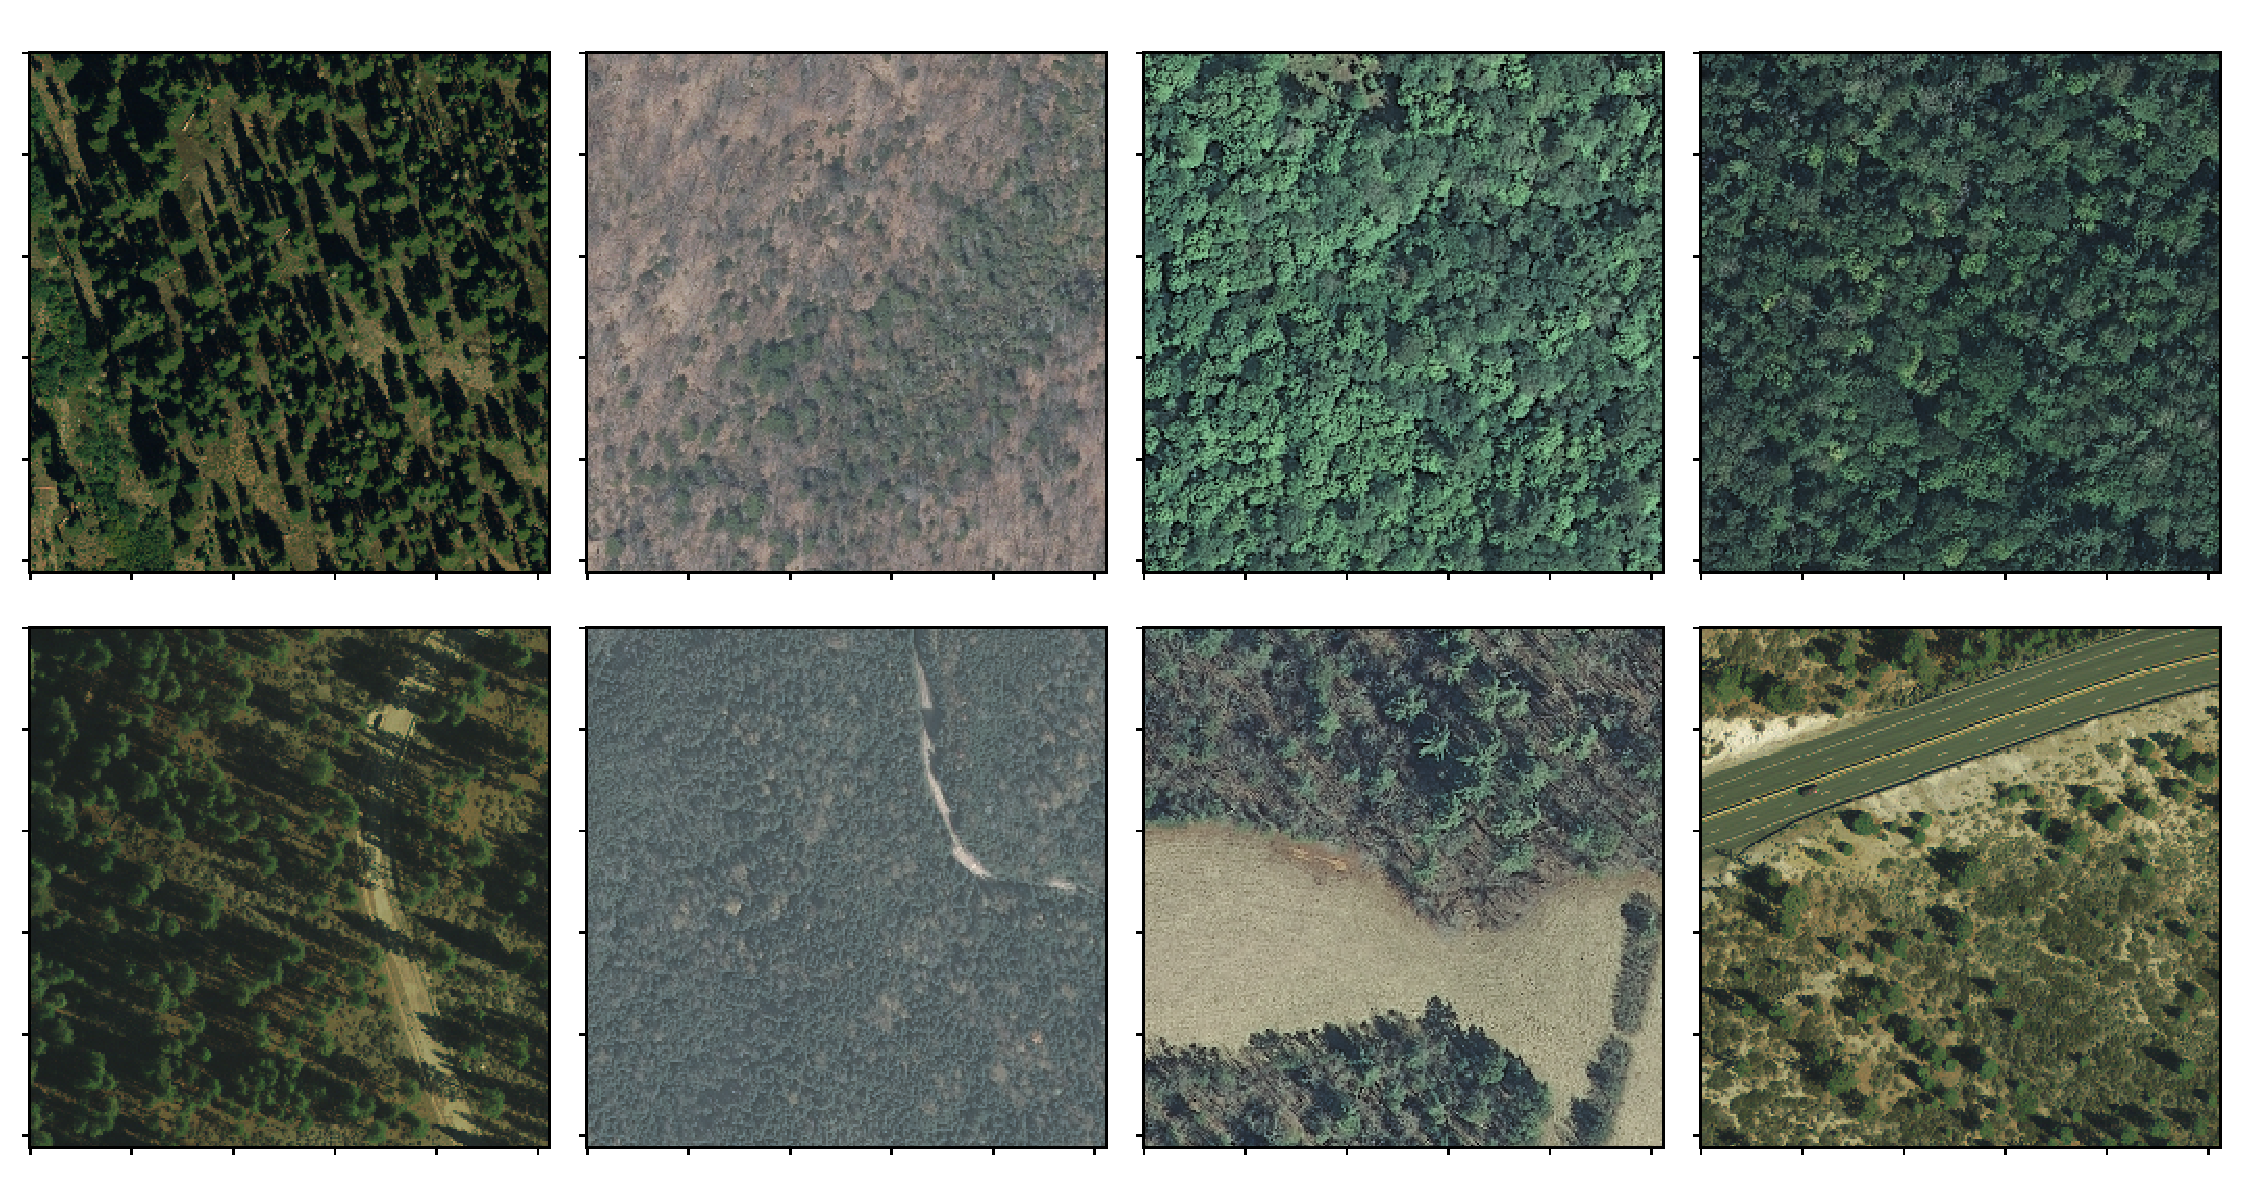
\includegraphics[width=1\textwidth]{Figures/forest-woodland_sample.pdf}
	\caption{\textbf{Example images of category Forest-woodland.} The images in the first row do not contain any human influence, while the images in the second row show influence by humans. The images in this figure have a size of $512\times512$ pixels and a resolution of $0.3$m per pixel.}
	\label{fig:forest-sample}
\end{figure}

\begin{figure}%[th]
	\centering
	\captionsetup{width=1\linewidth}
	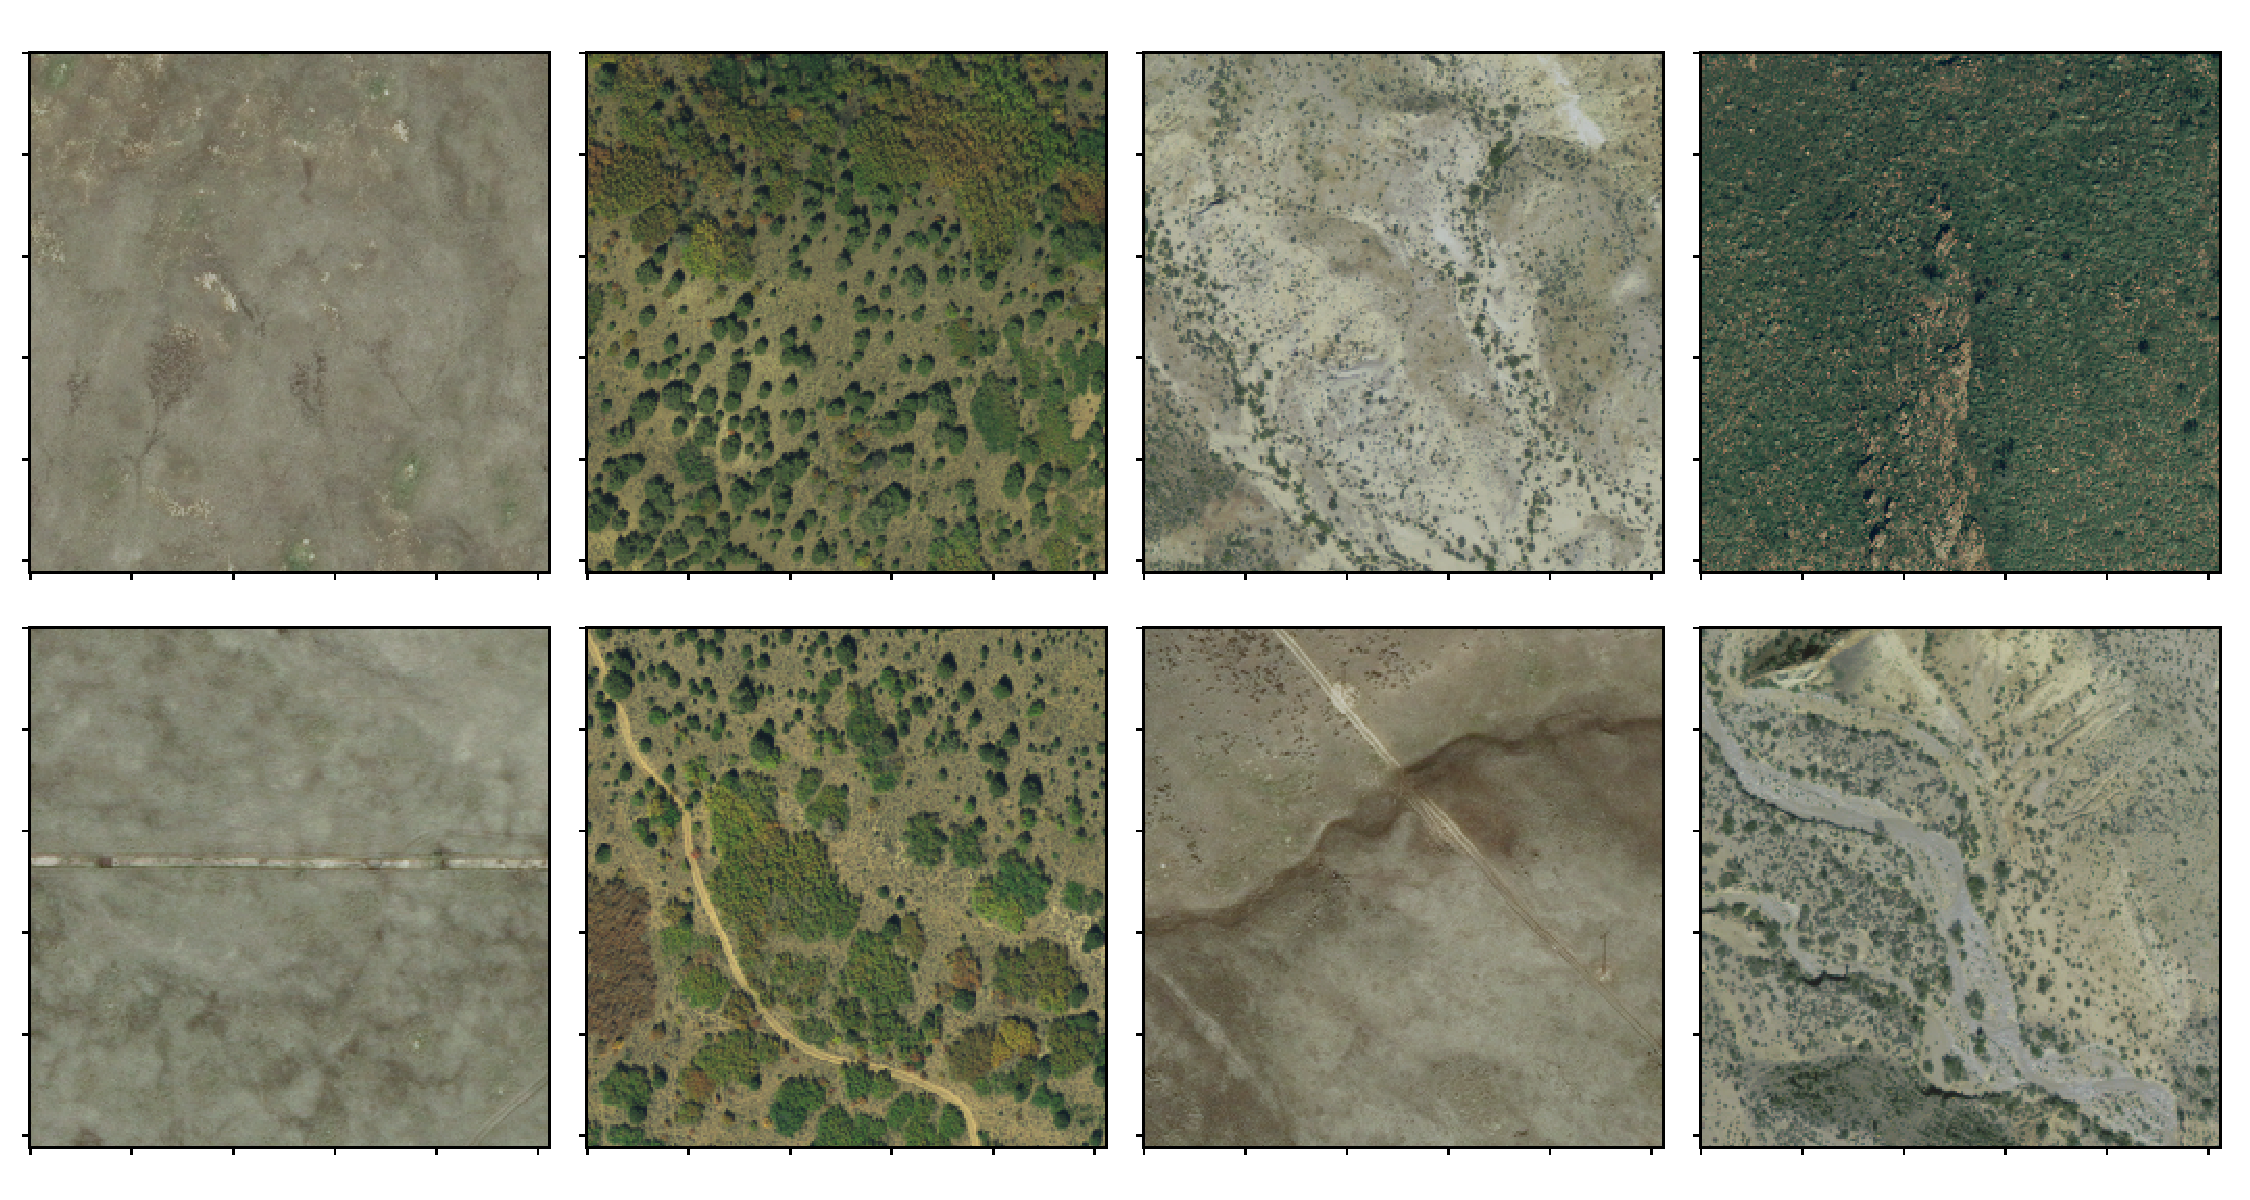
\includegraphics[width=1\textwidth]{Figures/semi-desert_sample.pdf}
	\caption{\textbf{Example images of category Semi-desert.} The images in the first row do not contain any human influence, while the images in the second row show influence by humans. The images in this figure have a size of $512\times512$ pixels and a resolution of $0.3$m per pixel.}
	\label{fig:desert-sample}
\end{figure}

Within each category of the processed images we labelled a selected portion of the images, by moving them into the folder with the respective label name. \textcolor{red}{SHOW FOLDER STRUCTURE SCHEMATICALLY}. When labelling 
we mainly followed two rules. First, we did not classify images that were ambigious, i.e. images that showed minimal human impact such as a small walking path. Second, we put a lot of effort in creating datasets that contain images of similar texture spread accross both classes. If we for example classified a set of images of a certain type of forest into the class with label 0 we classified another set of images with a similar type of forest, but containing a building or a street, into the class with label 1. We followed the latter rule for all categories except Agriculture. The Agriculture images all show human influence.
By sticking to these rules, we are able to guarantee that the algorithm learns features that relate purely to the human impact. 

In Figures \ref{fig:agriculture_sample} - \ref{fig:desert-sample} we display sample images for each of the four categories Agriculture, Shrubland-grassland, Forest-woodland and Semi-desert. These images belong to the dataset with 0.3m resolution per pixel. Note that in the Figs. \ref{fig:shrubland_sample} - \ref{fig:desert-sample} the first row represents images of label 0 and the second row shows images that belong to label 1. As mentioned above, the images in Fig.~\ref{fig:agriculture_sample} all contain human influence. Overall, we classified 

\begin{figure}%[th]
	\centering
	\captionsetup{width=1\linewidth}
	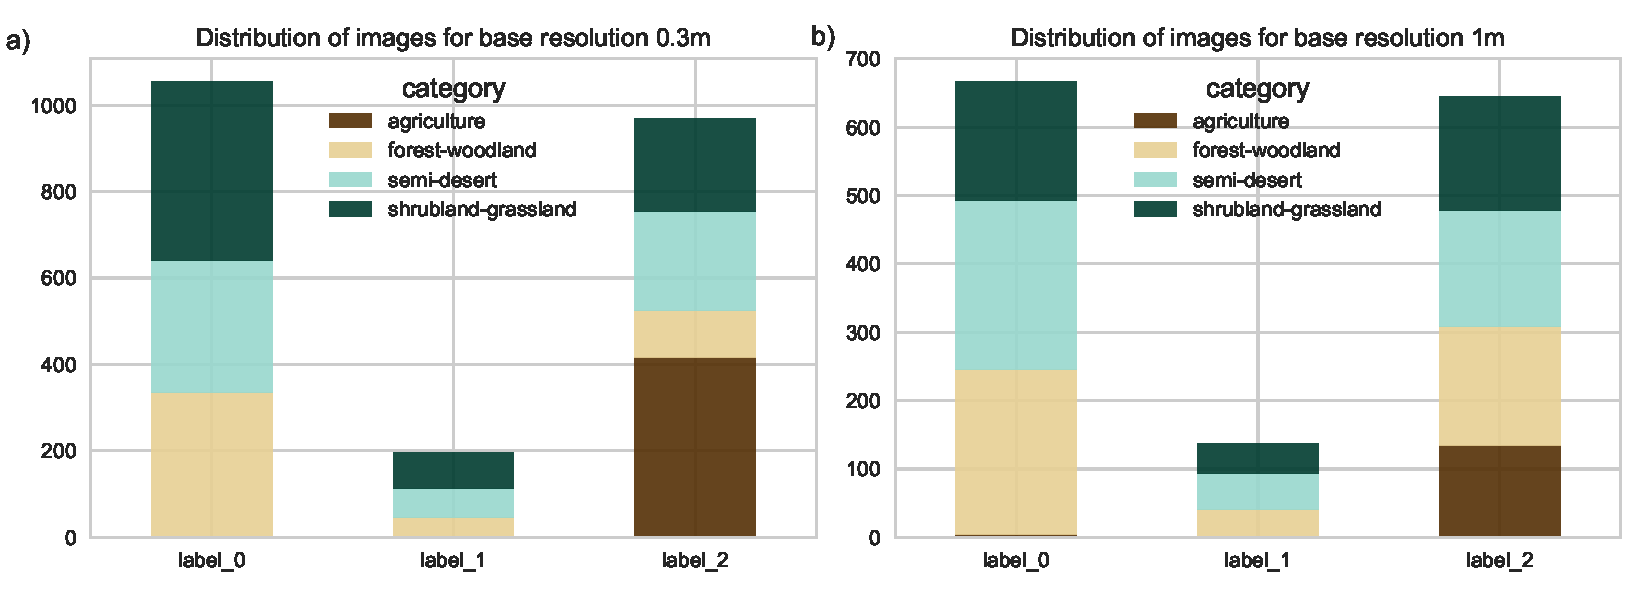
\includegraphics[width=1\textwidth]{Figures/imstats.pdf}
	\caption{\textbf{Image statistics.} }
	\label{fig:imstats}
\end{figure}

\begin{figure}%[th]
	\centering
	\captionsetup{width=1\linewidth}
	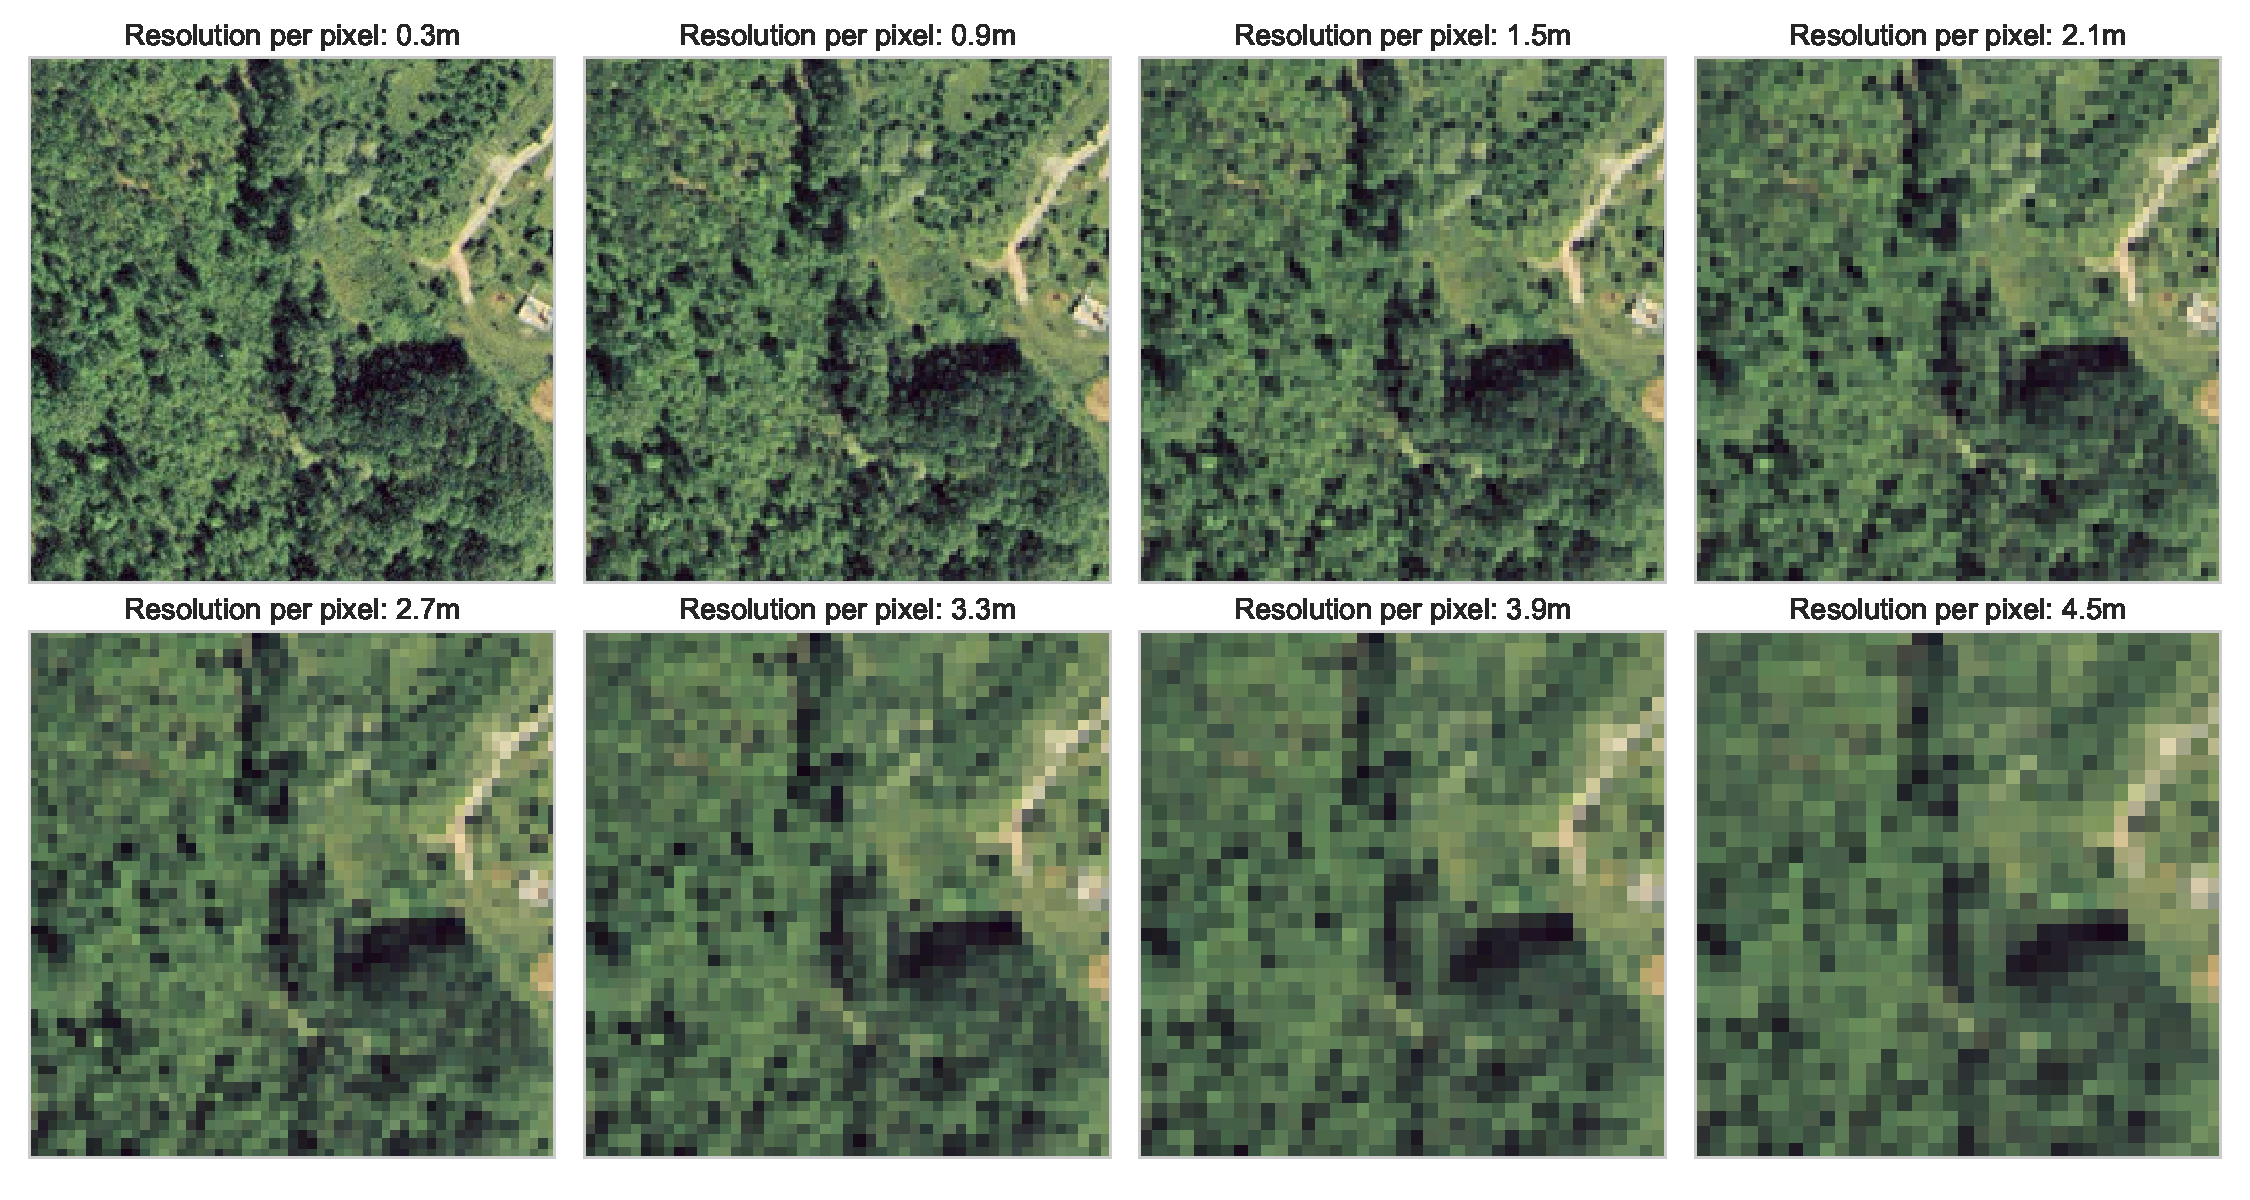
\includegraphics[width=1\textwidth]{Figures/demo_degrade.pdf}
	\caption{\textbf{Demo image resampling.} }
	\label{fig:degrade}
\end{figure}


\begin{itemize}
\item Image statistics 
\item Image degradation



\end{itemize}

%----------------------------------------------------------------------------------------
